\documentclass[12pt]{article}  % default square logo

\usepackage[margin=2.8cm]{geometry}
\usepackage{setspace}
\usepackage{mathptmx} % Times font
\usepackage[utf8]{inputenc}

% handles ~ in url
\usepackage{hyperref}

% center captions
\usepackage[justification=centering]{caption}

% code listing
\usepackage{listings}
\usepackage{xcolor}

% packages for drawing
\usepackage{tikz}
\usetikzlibrary{graphs}     % create graphs

% for warning box
\usepackage{pifont,mdframed}
\usepackage{framed}


%%%%%%%%%%%%%%%%%%%%%%%%%%%%%%%%%%%%%%%%%%%%%%%%%%%%%%%%%%%%%%%%%%%%%%%%%%%%%%%%%%%%%%%%%

\onehalfspacing

%% styles for filter graph
\tikzstyle{filter} = [rectangle, draw, font=\small, text centered, rounded corners, minimum height=2em, node distance=3cm, minimum width=4em]

%% set code styles

\definecolor{dkgreen}{rgb}{0,0.6,0}
\definecolor{gray}{rgb}{0.5,0.5,0.5}
\definecolor{mauve}{rgb}{0.58,0,0.82}

\lstset{
  frame=tb,
  language=scala,
  aboveskip=3mm,
  belowskip=3mm,
  showstringspaces=false,
  columns=flexible,
  basicstyle={\small\ttfamily},
  numbers=none,
  numberstyle=\tiny\color{gray},
  keywordstyle=\color{blue},
  commentstyle=\color{dkgreen},
  stringstyle=\color{mauve},
  breaklines=true,
  breakatwhitespace=true,
  tabsize=3,
}

%% warning box

\newenvironment{warning}
               {\par\begin{mdframed}[linewidth=1pt,linecolor=red!20,backgroundcolor=yellow!40]%
                 \begin{list}{}{\leftmargin=1cm
                     \labelwidth=\leftmargin}\item[\Large\ding{43}]}
               {\end{list}\end{mdframed}\par}

\newenvironment{info}
               {\par\begin{mdframed}[linewidth=1pt,backgroundcolor=blue!20!white]%
                 \begin{list}{}{\leftmargin=1cm
                     \labelwidth=\leftmargin}\item[\Large\ding{46}]}
               {\end{list}\end{mdframed}\par}

%%%%%%%%%%%%%%%%%%%%%%%%%%%%%%%%%%%%%%%%%%%%%%%%%%%%%%%%%%%%%%%%%%%%%%%%%%%%%%%%%%%%%%%%%
\begin{document}

\begin{titlepage}

  \begin{center}

    %% \vspace{20cm}
    \vspace*{3\baselineskip}
    % Title
    {\Large \bfseries Programming Guide for TradingSimulation \\[0.4cm] }

    % Author and supervisor
    \noindent
    TradingSimulation Developer Team \\[4cm]

    \begin{framed}
    Project of Big Data Course \\
    Professor: Christoph Koch \\
    \end{framed}

    \noindent
    Lausanne, Academic Year 2014 - 2015 \\[1cm]

    % Upper part of the page. The '~' is needed because \\
    % only works if a paragraph has started.
    
\includegraphics[width=0.8\textwidth]{img/epfl}~\\[1cm]

    \vfill

    % Bottom of the page
    {\large \today}

  \end{center}

\end{titlepage}

\subsection*{Preface}

The targeted audience of this documentation is developers who want to use the TradingSimulation framework to experiment with algorithmic trading or contribute to the TradingSimulation project. The readers should have some background in algorithmic trading or have access to expertises of the field. The reader should also be familiar with programming in Scala.


\pagenumbering{Roman}
\tableofcontents

\pagenumbering{arabic}

%!TEX root = ../guide.tex

\section{Introduction}
\label{sec:1}

This section introduces the functionalities, use cases and architecture of the TradingSimuation framework.

\subsection{What's TradingSimulation}

TradingSimulation is an open source\footnote{\url{https://github.com/merlinND/TradingSimulation}} algorithmic trading framework based on Scala\footnote{\url{http://scala-lang.org}}. The framework provides a lot of standardized components, which can be easily composed by the programmers with a few lines of Scala code to do various experiments related to algorithmic trading.

Following are a list of use cases of TradingSimulation:

\begin{itemize}
\item Simulation of multiple traders in a virtual market
\item Evaluation of a trading algorithm against live Forex data
\item Evaluation of a trading algorithm against live Bitcoin data
\item Evaluation of a trading algorithm based on historical market data
\end{itemize}

\subsection{The Architecture of TradingSimulation}

The design of TradingSimulation is based on the \emph{Pipes and Filters}\footnote{\url{http://www.cs.olemiss.edu/~hcc/csci581oo/notes/pipes.html}} architectural pattern, which results in a very high level of modularity, extensibility and reusability of the framework.

In the terminology of \emph{Pipes and Filters}, the standard components provided by the TradingSimulation framework are called \emph{filters}. The programmers can select appropriate filters and connect them properly according to the specific experiment purpose. Each configuration of filters is called a \emph{filter graph}.

Figure~\ref{fig-filter-graph} is an example filter graph of TradingSimulation. In the filter graph, there are six inter-connected filters.


\begin{figure}
  \centering
  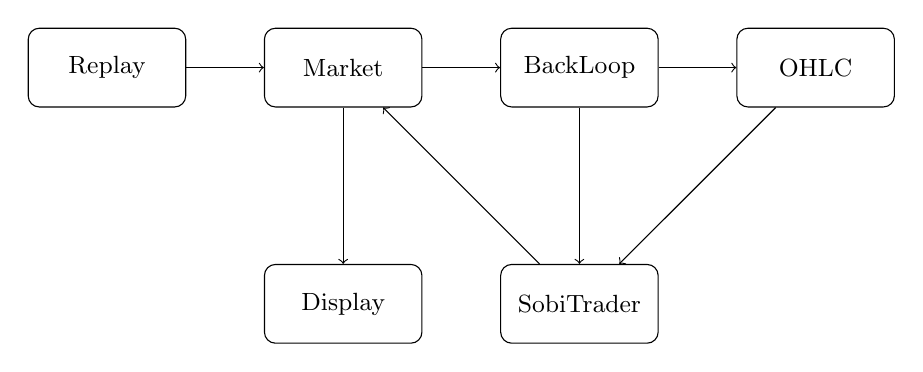
\begin{tikzpicture}[every node/.style={rectangle, draw, font=\small, text centered, rounded corners, node distance=3cm, minimum height=1cm, minimum width=2cm}]
    \node (Replay) {Replay};
    \node [right of=Replay] (Market) {Market};
    \node [right of=Market] (BackLoop) {BackLoop};
    \node [right of=BackLoop] (OHLC) {OHLC};
    \node [below of=BackLoop] (SobiTrader) {SobiTrader};
    \node [below of=Market] (Display) {Display};

    \graph [grow right=3cm] {
      (Replay) -> (Market) -> { (BackLoop) -> { (OHLC) -> (SobiTrader), (SobiTrader) }, (Display) };
      { (SobiTrader) } -> (Market);
    };
  \end{tikzpicture}
  \centering
  \caption{A Filter Graph in TradingSimulation}
  \label{fig-filter-graph}
\end{figure}

The functions of the filters in Figure~\ref{fig-filter-graph} are explained as follows:

\begin{itemize}
\item{Replay}: Read historical market order data from file system and send them one by one at a constant rate to connected filters. Replay is also called \emph{source filter}, as it doesn't have any input from other filters.
\item{Market}: Receive market orders, create transactions from matching bid and ask orders according to the configured market rules, and send transaction data to connected filters.
\item {BackLoop}: It's a utility filter, which sends everything it receives from input to output.
\item {OHLC}: It receives transaction data and send the prices of Opening, Highest, Lowest and Closing once a time in a configured interval.
\item {Display}: As its name suggests, this filter shows the data it receives in the terminal. It's also called \emph{sink filter}, as it doesn't send any data to other filters.
\item {SobiTrader}: This filter is a trader who employs the \emph{Static Order Book Imbalance}(SOBI) trading strategy. It receives market data such as orders, transactions and OHLC, and sends bid or ask orders to the \emph{Market}.
\end{itemize}

\subsection{A Simple Example}

Following code snippet is intended to give you some feel on how to create and run a filter graph in TradingSimulation.

\lstinputlisting[language=Scala]{code/simple.scala}

As you see in the code, it first creates a component builder, then uses the builder to create various  components, connects the components, and finally starts the graph.

All usages of TradingSimulation have the same form of code as shown in the code snippet, the difference lies in what components are created, what parameters are configured for components, and how components are connected.

For more and complete examples, please check our code repository here\footnote{\url{https://github.com/merlinND/TradingSimulation/tree/master/ts/src/main/scala/ch/epfl/ts/example}}.

\section{Components}
\label{sec:2}

This section introduces each component in detail, including  what data they expect, what data they output, what parameters can be set. After reading this section, you should able to select appropriate components for a specific algorithmic trading purpose, parameterize and connect them correctly.

\subsection{Define a Component}

In TradingSimulation, each component is an Akka\footnote{\url{http://akka.io}} actor. This can be seen from following code snippet, in which the abstract class \emph{Component} indirectly extends the trait \emph{Actor} in Akka. All concrete components extend \emph{Component}.

\begin{lstlisting}[language=Scala]
  trait Receiver extends Actor {
    def receive: PartialFunction[Any, Unit]

    def send[T: ClassTag](t: T): Unit
    def send[T: ClassTag](t: List[T]): Unit
  }

  abstract class Component extends Receiver {
    def start: Unit = {}

    def stop: Unit = {}

    def receiver: PartialFunction[Any, Unit]
  }
\end{lstlisting}

The framework defines three standard methods for every concrete component class:

\begin{itemize}
\item{start}: concrete components can override this method to do custom initialization.
\item{stop}: concrete components can override this method to release resources.
\item{receiver}: concrete components override this method to receive and handle messages.
\end{itemize}

The data transer between different components is in the form of Akka messages. Concrete component classes have to override the method \emph{receiver} in order to handle the messages they are interested in.

To send a message, a concrete component class can call one of the two \emph{send} methods defined in \emph{Receiver}. The two \emph{send} methods have default implementation in \emph{Component}, a concrete component class should not override them.

Following code snippet illustrates a very simple component which just prints and forwards every message it receives.

\begin{lstlisting}[language=Scala]
  class BackLoop extends Component {
    override def receiver = {
      case m =>
        println(m)
        send(m)
    }
  }
\end{lstlisting}

\subsubsection{Create Instances of Components}

To create an instance of a component, we have to first create a \emph{component builder} as follows:

\begin{lstlisting}[language=Scala]
val builder = new ComponentBuilder("test")
\end{lstlisting}

Now suppose we have a Component \emph{Arbitrageur} defined as follows:

\begin{lstlisting}[language=Scala]
  class Arbitrageur(id: Long, delta: Double, volume: Double) extends Component
  {
    //...
  }
\end{lstlisting}

Then we can create an instance of \emph{Arbitrageur} with following code snippet:

\begin{lstlisting}[language=Scala]
  val props = Props(classOf[Arbitrageur], 111L, 1, 50)
  val arbitrageur = builder.createRef(props, "arbitrageur")
\end{lstlisting}

As you can see in the code snippet above, first we create an instance of \emph{Props}\footnote{\url{http://doc.akka.io/api/akka/2.3.1/index.html\#akka.actor.Props}}. The first argument to \emph{Props} is the class we want to instantiate, and the remaining arguments are exactly the parameters that the constructor of the class \emph{Arbitrageur} expects.

\emph{builder.createRef} then takes \emph{props} and a name for the component to create an instance of the component. Note that the return value of \emph{builder.createRef} is a pointer to an instance of \emph{ComponentRef} instead of \emph{Arbitrageur}.

We have learned how to created instances of components, next let's see how to connect them.

\begin{info}
Internally, \emph{builder.createRef} will call \emph{actorOf} on an instance of \emph{ActorSystem} to create an instance of the component. The whole process seems a little awkward, but that's how Akka works. If you ever have a chance to checkout Akka(\href{http://akka.io}{akka.io}), you'll find it's worth the pain.
\end{info}

\subsubsection{Connect Components}

To connect an upstream component A to a downstream component B, we need to specify what types of messages B expects to receive from A. During the running A would only send messages of the specified types to B. For example, in the following code snippet, \emph{sobiTrader} will only send \emph{LimitBidOrder} messages to \emph{market}, and only send \emph{LimitAskOrder} messages to \emph{display}.

\begin{lstlisting}[language=Scala]
  sobiTrader -> (market, classOf[LimitBidOrder])
  sobiTrader -> (display, classOf[LimitAskOrder])
\end{lstlisting}

A downstream component can register as many message types as the upstream component can provide. For example, in the following code snippet \emph{sobiTrader} would send both \emph{LimitBidOrder} and \emph{LimitAskOrder} messages to \emph{market}.

\begin{lstlisting}[language=Scala]
  sobiTrader -> (market, classOf[LimitBidOrder], classOf[LimitAskOrder])
\end{lstlisting}

If a downstream component registers a message type that the upstream component can't provide, the registration has no effect. In practice, it's important to check carefully what messages a component can receive and provide.

Following list are all the types messages that are exchanged between components:

\begin{itemize}
\item Transaction
\item LimitBidOrder
\item LimitAskOrder
\item MarketBidOrder
\item MarketAskOrder
\item DelOrder
\item Quote
\item OHLC
\item MA
\end{itemize}

\subsection{Simulators}

Details of various simulators

\begin{itemize}
\item MarketSimulator
\item MarketFxSimulator
\end{itemize}

\subsection{Indicators}

Details various indicators

\begin{itemize}
\item MA
\item EMA
\item SMA
\item OHLC
\end{itemize}

\subsection{Traders}

Details of various traders

\begin{itemize}
\item Arbitrageur
\item DoubleCrossOverTrader
\item DoubleEnvelopeTrader
\item SimpleFXTrader
\item SimplerTrader
\item SobiTrader
\item TransactionVmapTrader
\end{itemize}

\subsection{Fetchers}

Details of various fecthers

\begin{itemize}
\item BitfinexFetcher
\item BitStampFetcher
\item BtceFetcher
\item CSVFetcher
\item TrueFXFetcher
\end{itemize}

\subsection{Utilities}

Other components

\begin{itemize}
\item Printer
\item Backloop
\item Replay
\item BatcherComponent
\end{itemize}

\section{Usage Scenarios}
\label{sec:3}

This section introduces how to use the framework for common usage scenarios. The examples are at the high level, no code is provided. If you want to refer to concrete examples in code, please refer to the package \emph{ch.epfl.ts.example} or check it out on \href{https://github.com/merlinND/TradingSimulation/tree/master/ts/src/main/scala/ch/epfl/ts/example}{Github}.

\subsection{Bitcoin Trading}

In this example, we demonstrate how to use the framework to experiment Bitcoin trading with the \emph{MovingAverageTrader} on live market data. The component graph of this application is as follows:

\noindent
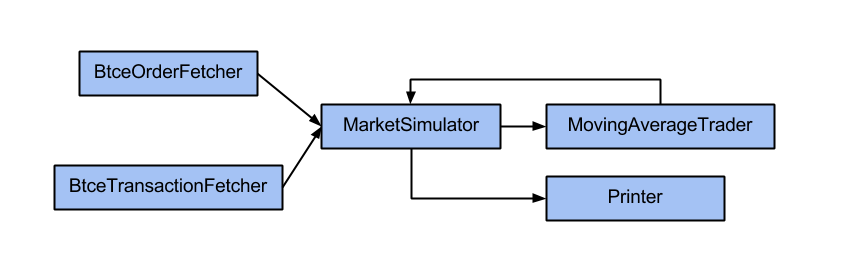
\includegraphics[width=\textwidth]{img/examples/btce}

The BTC-E fetchers get orders and transactions from \url{btc-e.com}, feed them to the market simulator. The market simulator generates transactions based on the bid and ask orders from the trader. The trader sends bid or ask orders to the market simulator based on the transactions received from the market simulator. The printer prints information about the market in the console.

\subsection{Forex Trading}

In this example, we demonstrate how to use the framework to experiment Forex trading with the \emph{MovingAverageTrader} on live Forex data. The component graph of this application is as follows:

\noindent
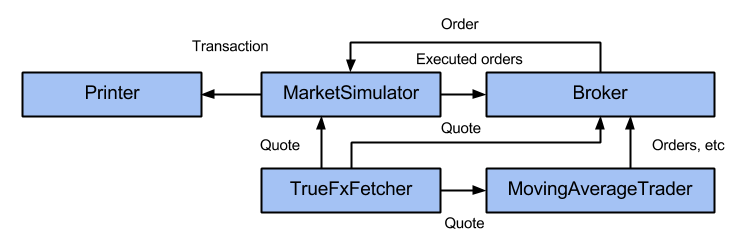
\includegraphics[width=\textwidth]{img/examples/forex-live}

In the component graph above, the fetcher gets live quotes data from \url{webrates.truefx.com}, and feeds them into the market simulator, trader and broker.

The trader makes sell and buy decisions based on the quotes received from the fetcher, and send them to the broker.

The broker receives orders from the trader, and forward them into the market simulator on behalf of the trader. Note that the usage of broker is optional, it's used here only for illustrating purpose.

The market simulator generates transactions based on the orders received from brokers, and sends the transaction result back to the broker.

\subsection{Replay}

In this example, we demonstrate how to use the framework to experiment Forex trading with the \emph{MovingAverageTrader} on history Forex data.

\noindent
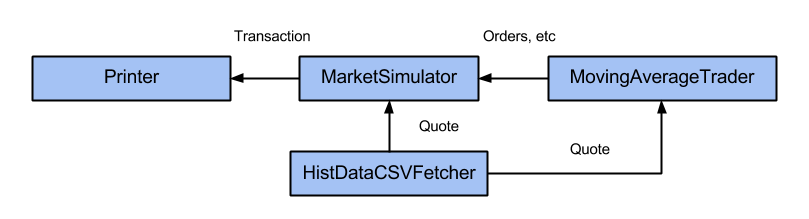
\includegraphics[width=\textwidth]{img/examples/forex-replay}

In the component graph above, the \emph{HistDataCSVFetcher} reads history quotes from CSV files, and send them to the market simulator and trader.

The trader produces ask or bid orders based on the quotes data, and sends them to the market simulator. The market simulator generates transactions based on the orders received from the trader.

The market simulator generates transactions based on received orders, and sends the transactions to the printer, which in turn prints them in the console.

%% \subsection{Simulation with Multiple Traders}

%% Multiple trader simulation in a virtual market.


\end{document}
